\documentclass[10pt]{article}
\usepackage[cp1251]{inputenc}
\usepackage[english]{babel}
\usepackage{url}
\usepackage{graphicx,DCCN2015_en}



\makeatletter
\c@page=1 % Number will be set by publisher.
          
\makeatother


% Proper title, should be and will be capitalized
\title{AUTHOR'S INSTRUCTIONS FOR THE PREPARATION OF CONTRIBUTIONS TO THE DCCN-2015 INTERNATIONAL CONFERENCE}
\author{N.~Surname1$^1$, N.~Surname2$^1$, N.~Surname3$^2$}
\company{$^1$ Affiliations1, City, Country\\$^2$ Affiliations2, City, Country}
\email{e-mail1, e-mail2, e-mail3}


%%%%%%%%%%%%%%%%%%%%%%%%%%%%%%%%

\begin{document}

\maketitle

%%%%%%%%%%%%%%%%%%%%%%%%%%%%%%%%%%%%%%%%%%%%%%%%%%%%%%%%%%%%%%
\begin{abstract}
Please type the short abstract here (no longer than 150 words) which summarizes the contents of the paper.
Do not use special characters, symbols, or math in your title
or abstract. The abstract should be written using the \emph{abstract} environment.
\keywords{We would like to encourage you to list your keywords within
the abstract section}
\end{abstract}
%%%%%%%%%%%%%%%%%%%%%%%%%%%%%%%%%%%%%%%%%%%%%%%%%%%%%%%%%%%%%%


\section{Introduction}

This demo file is intended to serve as a ``starter file'' for
the DCCN-2015 papers produced under \LaTeX.

The authors should submit up to 8 pages of the full-text paper. Use reduced B5
(170 x 240 mm) format of the paper. Margins: top 20 mm, bottom
30 mm, right 24 mm, left 24 mm. Text height is 185 mm, width is
120 mm. Authors are strongly recommended to fill the last page
of the paper at least 2/3 of a sheet. Please, do not use page
numbering in your paper. Actually, the authors don't have to be bothered about margins or suchlike,
because all the page geometry parameters are already set up in the DCCN2015\_en.sty style file.


\subsection{Subsection heading here}

Subsection text here. Maximum level of depth allowed for defining sections is 2.



\section{Submitted paper}

The full source text using \TeX{} as well as all auxiliary
materials, namely,
\begin{itemize}
  \item .tex file,
  \item pictures in .pdf (or .eps) format (if available),
  \item the paper in pdf format
\end{itemize}
have to be submitted as a zip-archive.

The name of the archive should be
\textbf{Surname1\_Surname2\_Surname3.zip}.

\section{Font}

Type the text of the paper in 10 points, regular. Each
paragraph is to be indented 5~mm, and their intervals must be 0
points before and after.

\section{Mathematical formulae and references}

To make references to mathematical expressions, it is
recommended to use \LaTeX{} mechanism. For example, the formula
given below
\begin{equation}
\label{eq:1}
P(n,t)=\frac{\partial^n B(t)}{\partial t^n}
\end{equation}
can be referred as \eqref{eq:1}.

\section{Theorems and proofs}

Theorems are defined like follows
\begin{thm}\label{thm1}
Text of the theorem.
\end{thm}

\begin{proof}
Proof of Theorem \ref{thm1}. If using such reference, you need
to recompile your paper with \LaTeX{} twice.
\end{proof}


\section{Figures and tables}

Figures should be provided in PDF or EPS format. Raster pictures have
to be made with maximal resolution (minimal 300 dots per inch).

\begin{figure}[h!]
   \centering
    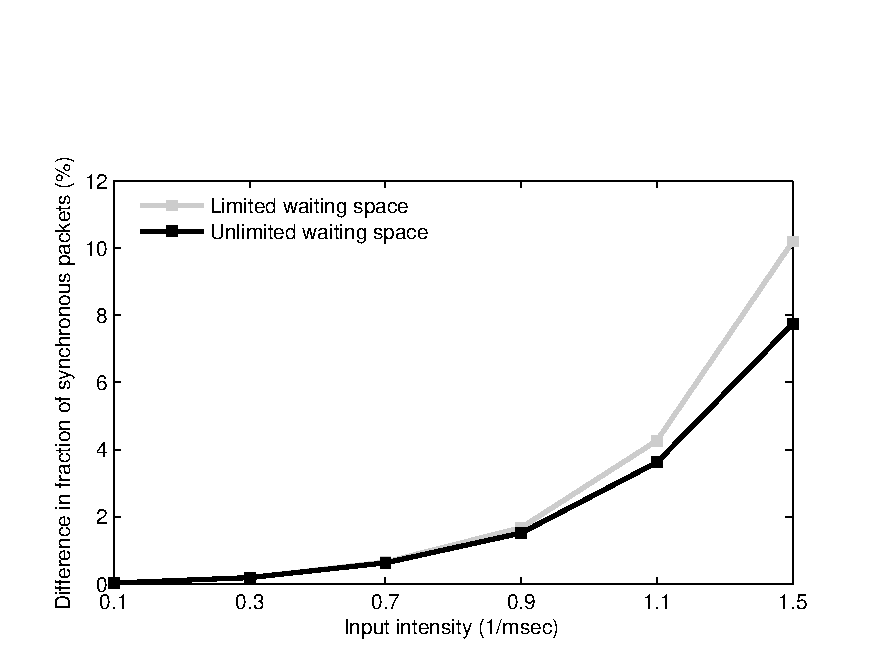
\includegraphics[width=\textwidth]{1.pdf} % or {1.eps} in case of EPS format of the picture
    \caption {Difference in fractions of synchronous packets for $W=16$.}
    \label{pic1}
\end{figure}

\begin{table}[h!]\begin{center}
\label{tab}
\begin{tabular}{|c||c|c|c||c||c|c|c|}\hline
  Parameter & T & E & $\Delta$, \% & Parameter & T & E & $\Delta$, \% \\ \hline \hline
  $\rho_{1}^{(1)}$ & 0,187 & 0,194 & 3,7 &  $\rho_{1}^{(2)}$ & 0,127 & 0,120 & 5,6 \\ \hline
  $\rho_{2}^{(1)}$ & 0,073 & 0,072 & 1,4 &  $\rho_{2}^{(2)}$ & 0,052 & 0,053 & 1,9 \\ \hline
  $\rho_{3}^{(1)}$ & 0,148 & 0,147 & 0,7 &  $\rho_{3}^{(2)}$ & 0,103 & 0,103 & 0,0 \\ \hline
  $\rho_{4}^{(1)}$ & 0,036 & 0,036 & 0,0 &  $\rho_{4}^{(2)}$ & 0,026 & 0,027 & 3,7 \\ \hline \hline
  $C^{(1)}$ & 0,479 & 0,476 & 0,6 & $C^{(2)}$ & 0,656 & 0,640 & 2,5 \\ \hline \hline
  $C_{1}^{*}$ & 0,341 & 0,339 & 0,6 & $C_{3}^{*}$ & 0,323 & 0,329 & 1,8 \\ \hline
  $C_{2}^{*}$ & 0,296 & 0,298 & 0,7 & $C_{4}^{*}$ & 0,286 & 0,286 & 0,0 \\ \hline
\end{tabular}\caption{Comparison of system parameters.}
\end{center}\end{table}

The figures and tables must be numbered, have a self-contained
caption and referred in the main text. Figure and table
captions are placed below the object and centered. Also, avoid
placing figures and tables before their first mention in the
text. Use the abbreviation "Fig." even at the beginning of a
sentence.

The authors are recommended not to use characters smaller than
9 point in figures. Do not use abbreviations in the titles
unless they are unavoidable.


\section{Conclusion}

Place a full list of references \cite{Bianchi00, VL02, neuts, GPSS, url} at the end of the paper. List
the references according to the order of their appearance in
the text.

%{\bf Acknowledgments.}

\begin{thebibliography}{99}
\bibitem{Bianchi00}  %% citation code
Bianchi G. Performance Analysis of the IEEE 802.11 Distributed
Coordination Function ~// IEEE Journal on Selected Areas in
Communications. 2000. V. 18. P.~535-547.

\bibitem{VL02} Vishnevsky V.~M., Lyakhov A.~I. IEEE 802.11
    Wireless LAN: Saturation Throughput Analysis with Seizing
    Effect Consideration
// Cluster Computing. 2002. V. 5. P. 133-144.

\bibitem{neuts} Neuts M.~F.  Structured Stochastic
    Matrices of M/G/1 Type and Their Applications. Marcel
    Dekker, New York, 1989.

\bibitem{GPSS} Schriber T.~J. Simulation using GPSS. John
    Wiley \& Sons, 1974.
    
\bibitem{url} National Center for Biotechnology Information, \url{http://www.ncbi.nlm.nih.gov}

\end{thebibliography}

\end{document}
